% vim: set spell spelllang=en tw=100 :

\documentclass[letterpaper]{article}
\usepackage[pass]{geometry}

\usepackage{ijcai13}
\usepackage{times}
\usepackage{complexity}
\usepackage{microtype}
\usepackage{gnuplot-lua-tikz}
\usepackage{amsmath}
\usepackage{amssymb}
\usepackage{placeins}
\usepackage{cleveref}
\usepackage{natbib}

% \usepackage{showframe}
\usepackage{lipsum}

\usetikzlibrary{decorations, decorations.pathreplacing, calc, backgrounds}

\definecolor{uofguniversityblue}{rgb}{0, 0.219608, 0.396078}

\definecolor{uofgheather}{rgb}{0.356863, 0.32549, 0.490196}
\definecolor{uofgaquamarine}{rgb}{0.603922, 0.72549, 0.678431}
\definecolor{uofgslate}{rgb}{0.309804, 0.34902, 0.380392}
\definecolor{uofgrose}{rgb}{0.823529, 0.470588, 0.709804}
\definecolor{uofgmocha}{rgb}{0.709804, 0.564706, 0.47451}
\definecolor{uofgsandstone}{rgb}{0.321569, 0.278431, 0.231373}
\definecolor{uofgforest}{rgb}{0, 0.2, 0.129412}
\definecolor{uofglawn}{rgb}{0.517647, 0.741176, 0}
\definecolor{uofgcobalt}{rgb}{0, 0.615686, 0.92549}
\definecolor{uofgturquoise}{rgb}{0, 0.709804, 0.819608}
\definecolor{uofgsunshine}{rgb}{1.0, 0.862745, 0.211765}
\definecolor{uofgpumpkin}{rgb}{1.0, 0.72549, 0.282353}
\definecolor{uofgthistle}{rgb}{0.584314, 0.070588, 0.447059}
\definecolor{uofgrust}{rgb}{0.603922, 0.227451, 0.023529}
\definecolor{uofgburgundy}{rgb}{0.490196, 0.133333, 0.223529}
\definecolor{uofgpillarbox}{rgb}{0.701961, 0.047059, 0}
\definecolor{uofglavendar}{rgb}{0.356863, 0.301961, 0.580392}

\title{Really Hard Instances for the Subgraph Isomorphism Problem}
\author{Ciaran McCreesh\thanks{This work was supported by the Engineering and Physical Sciences
    Research Council [grant number EP/K503058/1]} \and Patrick Prossser \and James Trimble \\
University of Glasgow, Glasgow, Scotland \\
c.mccreesh.1@research.gla.ac.uk}

\begin{document}

\maketitle

\begin{abstract}
    We show how to generate ``really hard'' random instances for variants of the subgraph
    isomorphism problem. For the non-induced variant of the problem, we locate a phase transition
    between satisfiable and unsatisfiable instances, with a corresponding complexity peak seen in
    three different solvers. For the induced variant of the problem, the behaviour is more
    complicated, with two phase transitions and an unexpectedly hard region in between. We show that
    this region remains hard when using pseudo-boolean and mixed integer encodings, and under
    reduction to the clique problem.
\end{abstract}

\section{Introduction}

The \emph{non-induced subgraph isomorphism problem} is to find an injective mapping from a given
pattern graph to a given target graph which preserves adjacency---in essence, we are ``finding a
copy of'' the pattern inside the target. The \emph{induced} variant of the problem additionally
requires that the mapping preserve non-adjacency, so there are no ``extra edges'' in the copy of the
pattern that we find. We illustrate both variants in \cref{figure:sip}.
Despite these problems being \NP-complete, modern practical subgraph isomorphism algorithms can
handle problem instances with many hundreds of vertices in the pattern graph, and up to ten thousand
vertices in the target graph \citep{Cordella:2004,Solnon:2010,Audemard:2014,McCreesh:2015}.

However, these algorithms cannot handle \emph{arbitrary} instances of this size. The experimental
evaluations of these algorithms were performed using a mix of real-world graphs, graphs that encode
biochemistry and computer vision problems, and randomly generated graph pairs. Using random
instances to evaluate algorithm behaviour can be beneficial, because it provides a way of generating
many instances cheaply, and reduces the risk of over-fitting when tuning design parameters. The
random instances used in each case came from common datasets (cite ??), which were generated by
taking a random subgraph of a random graph (using various models, including scale-free and bounded
degree) and permuting the vertices.  This is not ideal: such instances are guaranteed to be
satisfiable, and so existing benchmark suites contain relatively few non-trivial unsatisfiable
instances. These instances also tend to be computationally fairly easy, with most of the difficulty
being in dealing with the size of the model.

However, generating non-trivial unsatisfiable random instances is not straightforward. Using a
pattern graph from one of the random suites with the ``wrong'' target graph tends to give either a
trivially unsatisfiable instance, or a satisfiable instance. (In particular, it is \emph{not} the
case that a relatively small random graph is unlikely to appear in a larger random graph.)

\begin{figure}[b]
    \centering
    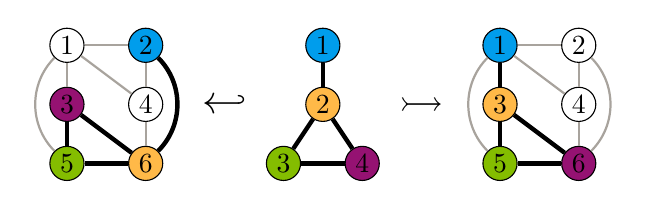
\begin{tikzpicture}[scale=0.5]
        \node [draw, circle, fill=uofgcobalt, inner sep=1.5pt] (Na) at (1,  0) {1};
        \node [draw, circle, fill=uofgpumpkin, inner sep=1.5pt] (Nb) at (1, -1.5) {2};
        \node [draw, circle, fill=uofglawn, inner sep=1.5pt] (Nc) at (0, -3) {3};
        \node [draw, circle, fill=uofgthistle, inner sep=1.5pt] (Nd) at (2, -3) {4};

        \draw [ultra thick] (Na) -- (Nb);
        \draw [ultra thick] (Nb) -- (Nc);
        \draw [ultra thick] (Nc) -- (Nd);
        \draw [ultra thick] (Nb) -- (Nd);

        \node [draw, circle, fill=uofgcobalt, inner sep=1.5pt] (N1) at (5.5,  0) {1};
        \node [draw, circle, fill=white, inner sep=1.5pt] (N2) at (7.5,  0) {2};
        \node [draw, circle, fill=uofgpumpkin, inner sep=1.5pt] (N3) at (5.5, -1.5) {3};
        \node [draw, circle, fill=white, inner sep=1.5pt] (N4) at (7.5, -1.5) {4};
        \node [draw, circle, fill=uofglawn, inner sep=1.5pt] (N5) at (5.5, -3) {5};
        \node [draw, circle, fill=uofgthistle, inner sep=1.5pt] (N6) at (7.5, -3) {6};

        \draw [thick, color=uofgsandstone!50] (N1) -- (N2);
        \draw [ultra thick] (N1) -- (N3);
        \draw [thick, color=uofgsandstone!50] (N1) -- (N4);
        \draw [thick, color=uofgsandstone!50] (N2) -- (N4);
        \draw [ultra thick] (N3) -- (N5);
        \draw [ultra thick] (N3) -- (N6);
        \draw [thick, color=uofgsandstone!50] (N4) -- (N6);
        \draw [ultra thick] (N5) -- (N6);
        \draw [thick, color=uofgsandstone!50] (N2) to [in=45, out=315] (N6);
        \draw [thick, color=uofgsandstone!50] (N1) to [in=135, out=225] (N5);

        \node [draw, circle, fill=white, inner sep=1.5pt] (M1) at (-5.5,  0) {1};
        \node [draw, circle, fill=uofgcobalt, inner sep=1.5pt] (M2) at (-3.5,  0) {2};
        \node [draw, circle, fill=uofgthistle, inner sep=1.5pt] (M3) at (-5.5, -1.5) {3};
        \node [draw, circle, fill=white, inner sep=1.5pt] (M4) at (-3.5, -1.5) {4};
        \node [draw, circle, fill=uofglawn, inner sep=1.5pt] (M5) at (-5.5, -3) {5};
        \node [draw, circle, fill=uofgpumpkin, inner sep=1.5pt] (M6) at (-3.5, -3) {6};

        \draw [thick, color=uofgsandstone!50] (M1) -- (M2);
        \draw [thick, color=uofgsandstone!50] (M1) -- (M3);
        \draw [thick, color=uofgsandstone!50] (M1) -- (M4);
        \draw [thick, color=uofgsandstone!50] (M2) -- (M4);
        \draw [ultra thick] (M3) -- (M5);
        \draw [ultra thick] (M3) -- (M6);
        \draw [thick, color=uofgsandstone!50] (M4) -- (M6);
        \draw [ultra thick] (M5) -- (M6);
        \draw [ultra thick] (M2) to [in=45, out=315] (M6);
        \draw [thick, color=uofgsandstone!50] (M1) to [in=135, out=225] (M5);

        \node [anchor=center, font=\Large] (A1) at (-1.5, -1.5) { $\hookleftarrow$ };
        \node [anchor=center, font=\Large] (A2) at ( 3.5, -1.5) { $\rightarrowtail$ };
    \end{tikzpicture}

    \caption{There is a non-induced isomorphism from the pattern graph, in the center, to the target
    on the right, mapping vertex 1 to 1, 2 to 3, 3 to 5 and 4 to 6. This is not an induced
    isomorphism, since there is an edge between 1 and 5 in the target but not between 1 and 3 in the
    pattern. The mapping from the pattern to the (same) target on the left, sending 1 to 2, 2 to 6, 3 to
    5 and 4 to 3, is both non-induced and induced.}
    \label{figure:sip}
\end{figure}

Here we present and evaluate a new method for creating random pattern/target pairs. This method
generates both satisfiable and unsatisfiable instances, and can produce computationally challenging
instances with only a few tens of vertices in the pattern, and 150 vertices in the target. Our work
builds upon the phase transition phenomena observed in satisfiability and graph colouring problems
first described by \citet{Cheeseman:1991} and \citet{Mitchell:1992}---?? cite later stuff and
explain really hard.

For subgraph isomorphism we have three relevant control parameters rather than one: we can
independently alter the edge probability of the pattern graph, the edge probability of the target
graph, and the relative orders (number of vertices) of the pattern and target graphs.  For
non-induced isomorphisms, with the correct choice of parameters we see results very similar to those
observed with boolean satisfiability problems: there is a phase transition from satisfiable to
unsatisfiable, and we see a complexity peak occur (with three different solvers) near this phase
transition.

For certain choices of parameter for induced isomorphisms, there are two phase transitions, going
from satisfiable to unsatisfiable, and then from unsatisfiable back to satisfiable. Again, when
going from satisfiable to unsatisfiable (from either direction), instances go from being trivial to
really hard to solve. However, each of the three solvers we tested also finds the central
unsatisfiable region to be really hard---this may be unexpected, since this region is not near a
phase transition and is apparently over-constrained. To show that this is not a simple weakness of
current subgraph isomorphism algorithms, we verify that this region is also hard when using use a
pseudo-boolean encoding, a mixed integer model, and under reduction to the clique problem.

?? We also explain why this behaviour is seen.

\subsection{Definitions}

Throughout, our graphs are unlabelled, undirected, and do not have any loops (vertices which are
adjacent to themselves). We write $\operatorname{V}(G)$ for the vertex set of a graph $G$. A
\emph{non-induced subgraph isomorphism} from a graph $P$ (called the \emph{pattern}) to a graph $T$
(called the \emph{target}) is an injective mapping from $\operatorname{V}(P)$ to
$\operatorname{V}(T)$ which preserves adjacency---that is, for every adjacent $v$ and $w$ in
$\operatorname{V}(P)$, the vertices $i(v)$ and $i(w)$ are adjacent in $T$. An \emph{induced subgraph
isomorphism} additionally preserves non-adjacency---that is, if $v$ and $w$ are not adjacent in $P$,
then $i(v)$ and $i(w)$ must not be adjacent in $T$. We use the notation $i : P \rightarrowtail T$
for a non-induced isomorphism, and $i : P \hookrightarrow T$ for an induced isomorphism.

The \emph{order} of a graph is the cardinality of its vertex set.  We write $G(v, p)$ for a random
graph with $v$ vertices, and an edge between each distinct pair of vertices with independent
probability $p$.

\subsection{Experimental Setup}

Our experiments were performed on systems with Intel Xeon E5-4650 v2 (Q1'14) CPUs and 768GBytes RAM
(although this much RAM was not needed), running Scientific Linux release 6.7.   ?? Software
versions. Clasp 3.1.3, Gurobi 6.0.5, Glasgow, LAD version 2, VFLib. Software was compiled using GCC
4.9.

?? Stuff about runtimes and recursive calls. We are not aiming to compare solvers; rather, we are
looking for solver-independent behaviour.

\section{Non-Induced Subgraph Isomorphisms}

\begin{figure}[t]
    \input{gen-graph-phase-transition.tex}
    \caption{With a fixed a pattern order of 20, a target order of 150, a target edge probability of 0.4, and
    varying pattern edge probability, we observe a phase transition and complexity peak in the non-induced
    variant. Each point represents one instance. The lines show mean search effort, and mean
    proportion satisfiable, using a larger sample size.}
    \label{figure:phase-transition}
\end{figure}

Suppose we arbitrarily decide upon a pattern order of 20, a target order of 150, and a fixed target
edge probability of 0.40. As we vary the pattern edge probability from 0 to 1, we would expect to see a shift from
entirely satisfiable instances (with no edges in the pattern, we can always find a match) to
entirely unsatisfiable instances (a maximum clique in this order and edge probability of target graph will
usually have between 9 and 12 vertices). Indeed, \cref{figure:phase-transition} shows that this is
the case: the line (and the points show a subset of the samples) ?? describe this a bit more, find
the 0.5 SAT mark.

Some stuff about the complexity peak in the Glasgow solver. This looks remarkably similar to random
3SAT problems---compare, for example, Figure 1 of \citet{LeytonBrown:2014}. In particular,
satisfiable instances tend to be easier but show greater variation than unsatisfiable instances, and
there are exceptionally hard satisfiable instances. (The parallel version of the Glasgow solver is
designed to eliminate these.)

\begin{figure}[tb]
    \input{gen-graph-non-induced.tex}
    \caption{Behaviour of algorithms on the non-induced variant. Each point is the average of ten
        runs. For each plot, the x-axis is the pattern edge probability and the y-axis is the target
        edge probability, both from 0 to 1. Along the top row, we show the proportion of instances which are
        satisfiable; the white bands shows the phase transitions. On the second row, we show the
        number of search nodes used by the Glasgow algorithm, on the third row, the number of
        search nodes used by the LAD algorithm, and the fourth, VF2; the dark regions indicate
        ``really hard'' instances.}
    \label{figure:non-induced}
\end{figure}

In the top row of \cref{figure:non-induced} we show the phase transition for the non-induced
variant, for patterns of order 10, 20 and 30, a target of order 150, and varying pattern (x-axis)
and target (y-axis) densities. Inside the orange region, at the bottom right of each plot, every
instance is unsatisfiable---here we are trying to find a dense pattern in a sparse target. In the
purple region, at the top left, every instance is satisfiable---we are looking for a sparse pattern
in a dense target (which is easy, since we only have to preserve adjacency, not non-adjacency). The
white band between the regions shows the location of the phase transition: here, roughly half the
instances are satisfiable.

On subsequent rows, we show the average difficulty of different algorithms.  We measure search
nodes. Cannot be used to compare performance of algorithms directly, but this does show that each
solver found the same set of instances difficult.

Satisfiable is easy, until very close to the phase transition. Unsatisfiable is much harder than
satisfiable. This is solver-independent, although VF2 is terrible.

?? Are unsatisfiable instances on the phase transition much harder than satisfiable ones?

In figure \cref{figure:phase-transition-bands} we show what happens for larger patterns.

\begin{figure}[tb]
    \input{gen-graph-phase-transition-bands.tex}
    \caption{The location of the phase transition, as the pattern grows. Shown are points where
    between 20\% and 80\% of instances are satisfiable.}
    \label{figure:phase-transition-bands}
\end{figure}

\subsection{Locating the Phase Transition}

?? Can we predict where that line is?

\lipsum[6]

\section{Induced Isomorphisms}

In \cref{figure:induced} we show the induced behaviour (modified Glasgow to include the complement
as a supplemental graph).

Pattern order 10, what we expect. Patterns 20 and 30 have large unsatisfiable regions in the middle,
but these remain hard. Pattern orders 14, 15 and 16 show the transition between the two styles.

Odd unsat with LAD at the top right (not EHPs), trivial for Glasgow: mapping a non-clique into a
clique. Glasgow looks at non-edges and can see immediately that no mapping is possible.

Note that this is solver-independent.

\begin{figure*}[t]
    \input{gen-graph-induced.tex}
    \caption{Behaviour of algorithms on the induced variant, shown in the style
    of \cref{figure:non-induced}. The second row shows a bound on the satisfiable region, by
    considering where a \emph{non-}induced isomorphism may also be a non-induced isomorphism between
    complement graphs.}\label{figure:induced}
\end{figure*}

\subsection{Predicting Induced Behaviour}

?? Graph showing the product of satisfiable with vertical flip, min (unsat) and max (sat) of search
nodes with vertical flip.

This suggests that we're not able to make use of adjacency and non-adjacency simultaneously.

\section{Other Encodings and Solvers}

\begin{figure*}[t]
    \input{gen-graph-sat.tex}
    \caption{Behaviour of other solvers on the induced variant on smaller graphs, shown in the style of
        \cref{figure:non-induced}. The second row shows the number of search nodes used by the Glasgow
        algorithm, the third row shows the number of decisions made by the Clasp pseudo-boolean solver,
        the fourth row shows the number of search nodes used by a clique encoding, and the fifth a mixed
        integer encoding with Gurobi.}\label{figure:alt}
\end{figure*}

Is this just a weakness of current subgraph isomorphism solvers? In \cref{figure:alt} we repeat the
experiments on smaller pattern and target graphs, using different solving techniques. Although these
techniques are not competitive in absolute terms, we wish to see if the same pattern of behaviour
occurs.

Direct pseudo-boolean encoding: variables for each assignment, cardinality constraints, edge and
non-edge constraints. We use the Clasp solver. We see that hard instances remain hard, including
inside the central region, and that the easy satisfiable instances remain easy. (Although not
presented here, we also tried an equivalent SAT encoding with the Glucose solver, and saw very
similar performance.)

\begin{figure}[tb]
    \centering
    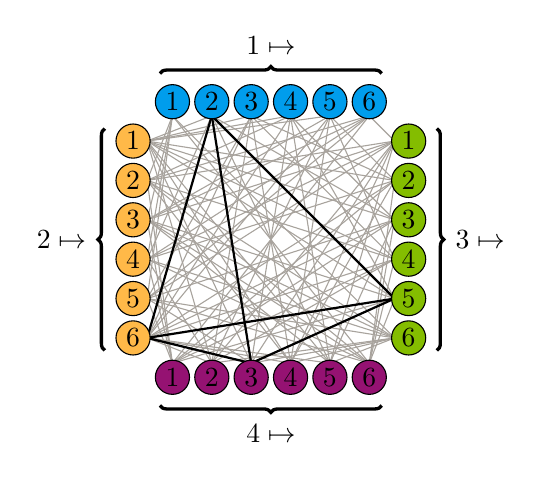
\begin{tikzpicture}[scale=0.5]

        \foreach \n in {1, ..., 6}{
            \node [draw, circle, fill=uofgcobalt, inner sep=1.5pt] (N1\n) at (\n, 0) {\n};
        }

        \draw [decorate, decoration={brace, raise=0.2cm}, very thick] (N11.north west) -- (N16.north
            east) node [midway, above=0.3cm] { $1 \mapsto$ };

        \foreach \n in {1, ..., 6}{
            \node [draw, circle, fill=uofgpumpkin, inner sep=1.5pt] (N2\n) at (0, -\n) {\n};
        }

        \draw [decorate, decoration={brace, raise=0.2cm, mirror}, very thick] (N21.north west) --
            (N26.south west) node [midway, left=0.3cm] { $2 \mapsto$ };

        \foreach \n in {1, ..., 6}{
            \node [draw, circle, fill=uofglawn, inner sep=1.5pt] (N3\n) at (7, -\n) {\n};
        }

        \draw [decorate, decoration={brace, raise=0.2cm}, very thick] (N31.north east) -- (N36.south
            east) node [midway, right=0.3cm] { $3 \mapsto$ };

        \foreach \n in {1, ..., 6}{
            \node [draw, circle, fill=uofgthistle, inner sep=1.5pt] (N4\n) at (\n, -7) {\n};
        }

        \draw [decorate, decoration={brace, raise=0.2cm, mirror}, very thick] (N41.south west) --
            (N46.south east) node [midway, below=0.3cm] { $4 \mapsto$ };

        \begin{scope}[on background layer]
            \draw [color=uofgsandstone!50] ($(N11)!0.8!(N11.south)$) -- ($(N22)!0.8!(N22.east)$);
            \draw [color=uofgsandstone!50] ($(N11)!0.8!(N11.south)$) -- ($(N23)!0.8!(N23.east)$);
            \draw [color=uofgsandstone!50] ($(N11)!0.8!(N11.south)$) -- ($(N24)!0.8!(N24.east)$);
            \draw [color=uofgsandstone!50] ($(N11)!0.8!(N11.south)$) -- ($(N25)!0.8!(N25.east)$);
            \draw [color=uofgsandstone!50] ($(N11)!0.8!(N11.south)$) -- ($(N36)!0.8!(N36.west)$);
            \draw [color=uofgsandstone!50] ($(N11)!0.8!(N11.south)$) -- ($(N46)!0.8!(N46.north)$);
            \draw [color=uofgsandstone!50] ($(N21)!0.8!(N21.east)$) -- ($(N12)!0.8!(N12.south)$);
            \draw [color=uofgsandstone!50] ($(N21)!0.8!(N21.east)$) -- ($(N32)!0.8!(N32.west)$);
            \draw [color=uofgsandstone!50] ($(N21)!0.8!(N21.east)$) -- ($(N42)!0.8!(N42.north)$);
            \draw [color=uofgsandstone!50] ($(N21)!0.8!(N21.east)$) -- ($(N13)!0.8!(N13.south)$);
            \draw [color=uofgsandstone!50] ($(N21)!0.8!(N21.east)$) -- ($(N33)!0.8!(N33.west)$);
            \draw [color=uofgsandstone!50] ($(N21)!0.8!(N21.east)$) -- ($(N43)!0.8!(N43.north)$);
            \draw [color=uofgsandstone!50] ($(N21)!0.8!(N21.east)$) -- ($(N14)!0.8!(N14.south)$);
            \draw [color=uofgsandstone!50] ($(N21)!0.8!(N21.east)$) -- ($(N34)!0.8!(N34.west)$);
            \draw [color=uofgsandstone!50] ($(N21)!0.8!(N21.east)$) -- ($(N44)!0.8!(N44.north)$);
            \draw [color=uofgsandstone!50] ($(N21)!0.8!(N21.east)$) -- ($(N15)!0.8!(N15.south)$);
            \draw [color=uofgsandstone!50] ($(N21)!0.8!(N21.east)$) -- ($(N35)!0.8!(N35.west)$);
            \draw [color=uofgsandstone!50] ($(N21)!0.8!(N21.east)$) -- ($(N45)!0.8!(N45.north)$);
            \draw [color=uofgsandstone!50] ($(N31)!0.8!(N31.west)$) -- ($(N22)!0.8!(N22.east)$);
            \draw [color=uofgsandstone!50] ($(N31)!0.8!(N31.west)$) -- ($(N42)!0.8!(N42.north)$);
            \draw [color=uofgsandstone!50] ($(N31)!0.8!(N31.west)$) -- ($(N23)!0.8!(N23.east)$);
            \draw [color=uofgsandstone!50] ($(N31)!0.8!(N31.west)$) -- ($(N43)!0.8!(N43.north)$);
            \draw [color=uofgsandstone!50] ($(N31)!0.8!(N31.west)$) -- ($(N24)!0.8!(N24.east)$);
            \draw [color=uofgsandstone!50] ($(N31)!0.8!(N31.west)$) -- ($(N44)!0.8!(N44.north)$);
            \draw [color=uofgsandstone!50] ($(N31)!0.8!(N31.west)$) -- ($(N25)!0.8!(N25.east)$);
            \draw [color=uofgsandstone!50] ($(N31)!0.8!(N31.west)$) -- ($(N45)!0.8!(N45.north)$);
            \draw [color=uofgsandstone!50] ($(N31)!0.8!(N31.west)$) -- ($(N16)!0.8!(N16.south)$);
            \draw [color=uofgsandstone!50] ($(N41)!0.8!(N41.north)$) -- ($(N22)!0.8!(N22.east)$);
            \draw [color=uofgsandstone!50] ($(N41)!0.8!(N41.north)$) -- ($(N32)!0.8!(N32.west)$);
            \draw [color=uofgsandstone!50] ($(N41)!0.8!(N41.north)$) -- ($(N23)!0.8!(N23.east)$);
            \draw [color=uofgsandstone!50] ($(N41)!0.8!(N41.north)$) -- ($(N33)!0.8!(N33.west)$);
            \draw [color=uofgsandstone!50] ($(N41)!0.8!(N41.north)$) -- ($(N24)!0.8!(N24.east)$);
            \draw [color=uofgsandstone!50] ($(N41)!0.8!(N41.north)$) -- ($(N34)!0.8!(N34.west)$);
            \draw [color=uofgsandstone!50] ($(N41)!0.8!(N41.north)$) -- ($(N25)!0.8!(N25.east)$);
            \draw [color=uofgsandstone!50] ($(N41)!0.8!(N41.north)$) -- ($(N35)!0.8!(N35.west)$);
            \draw [color=uofgsandstone!50] ($(N41)!0.8!(N41.north)$) -- ($(N16)!0.8!(N16.south)$);
            \draw [color=uofgsandstone!50] ($(N12)!0.8!(N12.south)$) -- ($(N33)!0.8!(N33.west)$);
            \draw [color=uofgsandstone!50] ($(N12)!0.8!(N12.south)$) -- ($(N24)!0.8!(N24.east)$);
            \draw [color=uofgsandstone!50] ($(N12)!0.8!(N12.south)$) -- ($(N45)!0.8!(N45.north)$);
            \draw [color=uofgsandstone!50] ($(N22)!0.8!(N22.east)$) -- ($(N14)!0.8!(N14.south)$);
            \draw [color=uofgsandstone!50] ($(N22)!0.8!(N22.east)$) -- ($(N34)!0.8!(N34.west)$);
            \draw [color=uofgsandstone!50] ($(N22)!0.8!(N22.east)$) -- ($(N44)!0.8!(N44.north)$);
            \draw [color=uofgsandstone!50] ($(N22)!0.8!(N22.east)$) -- ($(N16)!0.8!(N16.south)$);
            \draw [color=uofgsandstone!50] ($(N22)!0.8!(N22.east)$) -- ($(N36)!0.8!(N36.west)$);
            \draw [color=uofgsandstone!50] ($(N22)!0.8!(N22.east)$) -- ($(N46)!0.8!(N46.north)$);
            \draw [color=uofgsandstone!50] ($(N32)!0.8!(N32.west)$) -- ($(N13)!0.8!(N13.south)$);
            \draw [color=uofgsandstone!50] ($(N32)!0.8!(N32.west)$) -- ($(N24)!0.8!(N24.east)$);
            \draw [color=uofgsandstone!50] ($(N32)!0.8!(N32.west)$) -- ($(N44)!0.8!(N44.north)$);
            \draw [color=uofgsandstone!50] ($(N32)!0.8!(N32.west)$) -- ($(N15)!0.8!(N15.south)$);
            \draw [color=uofgsandstone!50] ($(N32)!0.8!(N32.west)$) -- ($(N26)!0.8!(N26.east)$);
            \draw [color=uofgsandstone!50] ($(N32)!0.8!(N32.west)$) -- ($(N46)!0.8!(N46.north)$);
            \draw [color=uofgsandstone!50] ($(N42)!0.8!(N42.north)$) -- ($(N13)!0.8!(N13.south)$);
            \draw [color=uofgsandstone!50] ($(N42)!0.8!(N42.north)$) -- ($(N24)!0.8!(N24.east)$);
            \draw [color=uofgsandstone!50] ($(N42)!0.8!(N42.north)$) -- ($(N34)!0.8!(N34.west)$);
            \draw [color=uofgsandstone!50] ($(N42)!0.8!(N42.north)$) -- ($(N15)!0.8!(N15.south)$);
            \draw [color=uofgsandstone!50] ($(N42)!0.8!(N42.north)$) -- ($(N26)!0.8!(N26.east)$);
            \draw [color=uofgsandstone!50] ($(N42)!0.8!(N42.north)$) -- ($(N36)!0.8!(N36.west)$);
            \draw [color=uofgsandstone!50] ($(N13)!0.8!(N13.south)$) -- ($(N34)!0.8!(N34.west)$);
            \draw [color=uofgsandstone!50] ($(N13)!0.8!(N13.south)$) -- ($(N44)!0.8!(N44.north)$);
            \draw [color=uofgsandstone!50] ($(N13)!0.8!(N13.south)$) -- ($(N25)!0.8!(N25.east)$);
            \draw [color=uofgsandstone!50] ($(N13)!0.8!(N13.south)$) -- ($(N26)!0.8!(N26.east)$);
            \draw [color=uofgsandstone!50] ($(N23)!0.8!(N23.east)$) -- ($(N15)!0.8!(N15.south)$);
            \draw [color=uofgsandstone!50] ($(N23)!0.8!(N23.east)$) -- ($(N35)!0.8!(N35.west)$);
            \draw [color=uofgsandstone!50] ($(N23)!0.8!(N23.east)$) -- ($(N45)!0.8!(N45.north)$);
            \draw [color=uofgsandstone!50] ($(N23)!0.8!(N23.east)$) -- ($(N16)!0.8!(N16.south)$);
            \draw [color=uofgsandstone!50] ($(N23)!0.8!(N23.east)$) -- ($(N36)!0.8!(N36.west)$);
            \draw [color=uofgsandstone!50] ($(N23)!0.8!(N23.east)$) -- ($(N46)!0.8!(N46.north)$);
            \draw [color=uofgsandstone!50] ($(N33)!0.8!(N33.west)$) -- ($(N14)!0.8!(N14.south)$);
            \draw [color=uofgsandstone!50] ($(N33)!0.8!(N33.west)$) -- ($(N25)!0.8!(N25.east)$);
            \draw [color=uofgsandstone!50] ($(N33)!0.8!(N33.west)$) -- ($(N45)!0.8!(N45.north)$);
            \draw [color=uofgsandstone!50] ($(N33)!0.8!(N33.west)$) -- ($(N26)!0.8!(N26.east)$);
            \draw [color=uofgsandstone!50] ($(N33)!0.8!(N33.west)$) -- ($(N46)!0.8!(N46.north)$);
            \draw [color=uofgsandstone!50] ($(N43)!0.8!(N43.north)$) -- ($(N14)!0.8!(N14.south)$);
            \draw [color=uofgsandstone!50] ($(N43)!0.8!(N43.north)$) -- ($(N25)!0.8!(N25.east)$);
            \draw [color=uofgsandstone!50] ($(N43)!0.8!(N43.north)$) -- ($(N36)!0.8!(N36.west)$);
            \draw [color=uofgsandstone!50] ($(N14)!0.8!(N14.south)$) -- ($(N35)!0.8!(N35.west)$);
            \draw [color=uofgsandstone!50] ($(N14)!0.8!(N14.south)$) -- ($(N45)!0.8!(N45.north)$);
            \draw [color=uofgsandstone!50] ($(N14)!0.8!(N14.south)$) -- ($(N26)!0.8!(N26.east)$);
            \draw [color=uofgsandstone!50] ($(N24)!0.8!(N24.east)$) -- ($(N16)!0.8!(N16.south)$);
            \draw [color=uofgsandstone!50] ($(N24)!0.8!(N24.east)$) -- ($(N36)!0.8!(N36.west)$);
            \draw [color=uofgsandstone!50] ($(N24)!0.8!(N24.east)$) -- ($(N46)!0.8!(N46.north)$);
            \draw [color=uofgsandstone!50] ($(N34)!0.8!(N34.west)$) -- ($(N15)!0.8!(N15.south)$);
            \draw [color=uofgsandstone!50] ($(N34)!0.8!(N34.west)$) -- ($(N26)!0.8!(N26.east)$);
            \draw [color=uofgsandstone!50] ($(N34)!0.8!(N34.west)$) -- ($(N46)!0.8!(N46.north)$);
            \draw [color=uofgsandstone!50] ($(N44)!0.8!(N44.north)$) -- ($(N15)!0.8!(N15.south)$);
            \draw [color=uofgsandstone!50] ($(N44)!0.8!(N44.north)$) -- ($(N26)!0.8!(N26.east)$);
            \draw [color=uofgsandstone!50] ($(N44)!0.8!(N44.north)$) -- ($(N36)!0.8!(N36.west)$);
            \draw [color=uofgsandstone!50] ($(N15)!0.8!(N15.south)$) -- ($(N26)!0.8!(N26.east)$);
            \draw [color=uofgsandstone!50] ($(N25)!0.8!(N25.east)$) -- ($(N16)!0.8!(N16.south)$);
            \draw [color=uofgsandstone!50] ($(N25)!0.8!(N25.east)$) -- ($(N36)!0.8!(N36.west)$);
            \draw [color=uofgsandstone!50] ($(N25)!0.8!(N25.east)$) -- ($(N46)!0.8!(N46.north)$);
            \draw [color=uofgsandstone!50] ($(N35)!0.8!(N35.west)$) -- ($(N46)!0.8!(N46.north)$);
            \draw [color=uofgsandstone!50] ($(N45)!0.8!(N45.north)$) -- ($(N26)!0.8!(N26.east)$);
            \draw [color=uofgsandstone!50] ($(N45)!0.8!(N45.north)$) -- ($(N36)!0.8!(N36.west)$);
            \draw [thick] ($(N12)!0.8!(N12.south)$) -- ($(N43)!0.8!(N43.north)$);
            \draw [thick] ($(N12)!0.8!(N12.south)$) -- ($(N35)!0.8!(N35.west)$);
            \draw [thick] ($(N12)!0.8!(N12.south)$) -- ($(N26)!0.8!(N26.east)$);
            \draw [thick] ($(N43)!0.8!(N43.north)$) -- ($(N35)!0.8!(N35.west)$);
            \draw [thick] ($(N43)!0.8!(N43.north)$) -- ($(N26)!0.8!(N26.east)$);
            \draw [thick] ($(N35)!0.8!(N35.west)$) -- ($(N26)!0.8!(N26.east)$);
        \end{scope}

    \end{tikzpicture}
    \caption{The association graph encoding of the induced version of \cref{figure:sip}. The clique
    of size four corresponds to the mapping sending pattern vertex 1 to target vertex 2, 2 to 6, 3
    to 5, and 4 to 3.}\label{figure:assoc}
\end{figure}

Clique encoding: association graph, a version of BBMC modified to solve the decision problem. The
hard instances in the central region remain hard. Additionally, some of the easy satisfiable
instances become hard. Possible weakness of clique algorithms for this kind of input.

MIP encoding with Gurobi.

?? \citep{Anton:2009}

?? \citep{Lipets:2009}

\section{Conclusion}

\bibliographystyle{named}
\bibliography{paper}

\end{document}
